% quantgrav.tex - working draft (skeleton).  Build:  make quantgrav   (writes build/quantgrav.pdf)
% Every number quoted in the text is a macro \qg... from build/quantgrav_numbers.tex, which models/paper_numbers.py writes from the models.
% Write negative numbers inside math mode ($...$) so that the minus sign is typeset as a minus.
\documentclass[11pt]{article}
\usepackage[T1]{fontenc}
\usepackage[utf8]{inputenc}
\usepackage{amsmath,amssymb,amsthm}
\usepackage{mathtools}
\usepackage[a4paper,margin=28mm]{geometry}
\usepackage{graphicx}
\usepackage{booktabs}
\usepackage{xcolor}
\usepackage{enumitem}
\usepackage{url}
\usepackage[hidelinks]{hyperref}
\graphicspath{{figures/}}
\IfFileExists{build/quantgrav_numbers.tex}{\input{build/quantgrav_numbers.tex}}{\PackageError{quantgrav}{Run models/paper_numbers.py first (make quantgrav does)}{}}

% labels of evidence, used in every result
\newcommand{\exact}{\textbf{\textsc{Exact}}}
\newcommand{\numeric}{\textbf{\textsc{Numeric}}}
\newcommand{\hypo}{\textbf{\textsc{Hypothesis}}}
\newcommand{\negres}{\textbf{\textsc{Negative}}}
\newcommand{\snap}{\textsuperscript{$\dagger$}}      % number copied from a snapshot, not recomputed by paper_numbers.py
\newcommand{\todo}[1]{\textcolor{red}{[TODO: #1]}}
\theoremstyle{definition}
\newtheorem{result}{Result}

\title{Hopf fibres of $E_8$, the Spectre monotile and the Chair44:\\
exact structure, negative results, and an abelian Wilson-loop probe}
\author{Working draft \\ \small Drafted with the help of Claude (Anthropic); not independently reviewed}
\date{\today}

\begin{document}
\maketitle

\begin{abstract}
\todo{write last. Draft: We collect finite, machine-checked computations that connect the Spectre aperiodic monotile, the Chair44 solid, the $E_8$
lattice with its Hopf fibres, and an abelian Wilson-loop analogue. The positive results are exact statements about root systems and lattices; the negative
results record what does not carry over (the Spectre inflation does not extend to $E_8$; the count $192$ matches only in shape); the Wilson-loop probe
shows how far one corner constant per corner reaches in a $U(1)$ analogue. We make no claim about quantum gravity.}
\end{abstract}

%------------------------------------------------------------------------------------------------------------------------------------
\section{Scope and conventions}\label{sec:scope}
\todo{what the paper is: a collection of finite computations with tests; what it is not: no physical claim, no proof of anything in the Wilson-loop programme.}
Every result carries one of the labels \exact\ (an identity or a finite enumeration, checked by a test that can fail), \numeric\ (a computed number on a
finite patch, with the tolerance stated), \negres\ (a natural expectation that the computation refutes) or \hypo\ (not shown). Numbers marked
$\dagger$ are copied from the output of another repository (Section~\ref{sec:wilson}) and are not recomputed by the code of this repository.
\todo{LLM-assistance disclosure in the wording the Wilson repository uses; reproduction: \texttt{make test}, \texttt{make quantgrav}.}

\begin{table}[h]
\centering\footnotesize
\begin{tabular}{@{}p{70mm}p{26mm}p{9mm}p{35mm}@{}}
\toprule
Result & Label & Section & Test module \\ \midrule
$\qgInscribed$ inscribed 24-cells and $\qgPartitions$ coset partitions of the 600-cell & \exact & \ref{sec:e8} & \texttt{hopf\_shells} \\
Ball window never splits a fibre; Voronoi window keeps all fibres whole & \exact/\numeric & \ref{sec:e8} & \texttt{fibre\_window}, \texttt{voronoi\_window} \\
$E_6$ and $A_2$ inside the fibres, $\qgRest=6\times27$ & \exact & \ref{sec:e8} & \texttt{e6\_fibres} \\
Spectre lift lattice is $A_2\oplus A_2\subset E_8$; every edge is a root & \exact & \ref{sec:tiles} & \texttt{spectre\_in\_e8} \\
The Spectre inflation does not extend to $E_8$ & \negres & \ref{sec:tiles} & \texttt{spectre\_in\_e8} \\
$\qgChairTips=24\times8$ Chair44 tips against the equatorial roots & \negres & \ref{sec:chair} & \texttt{chair\_e8\_192} \\
Corner locality, placement dependence, gauge, block size ($U(1)$) & \numeric$^\dagger$ & \ref{sec:wilson} & Wilson repository \\
\bottomrule
\end{tabular}
\caption{Summary of results. \todo{complete once the sections are drafted.}}
\end{table}

%------------------------------------------------------------------------------------------------------------------------------------
\section{Background}\label{sec:background}
\subsection{The Spectre and its lift}
\todo{Spectre \cite{smith2023}; edges are unit vectors at multiples of $30^\circ$; red and green hexagonal lattices; the lift lattice $\mathbb{Z}[\zeta_{12}]=\mathbb{Z}^4$ (the lift of Ch\'eritat and Ma \cite{cheritat2023}; the identification with $\mathbb{Z}[\zeta_{12}]$ is made in this repository's \texttt{lift4d.py}).}
\subsection{The Chair44}
\todo{the solid, its \qgChairPanels\ panels and \qgChairTips\ pyramid tips; data source and licence (\texttt{models/data/README.md}).}
\subsection{\texorpdfstring{$E_8$}{E8}, the icosians and the Hopf fibres}\label{sec:bg-e8}
Let $\mathbb{H}$ denote the Hurwitz order, the integer and half-integer quaternions, and $2T\subset\mathbb{H}$ its $24$ units. We use the standard
model of $E_8$ as the set of pairs $(a,b)\in\mathbb{H}^2$ with $a-b\in(1+i)\mathbb{H}$, scaled so that the roots have norm $|a|^2+|b|^2=2$. There are
\qgRoots\ roots: $192$ with $|a|=|b|=1$ (the \emph{equatorial} roots) and $48$ with one coordinate zero (the \emph{poles}, $24$ in each coordinate).
Right multiplication $(a,b)\mapsto(a\ell,b\ell)$ by $\ell\in 2T$ is an automorphism of the lattice. Its orbits are the \emph{fibres}: the roots fall
into \qgFibres\ fibres of \qgFibreSize\ roots, and each fibre is the vertex set of a $24$-cell. The Hopf map
$(a,b)\mapsto(|a|^2-|b|^2,\,2a\bar b)\in\mathbb{R}\times\mathbb{H}$ is constant on a fibre, because $(a\ell)\overline{(b\ell)}=a\bar b$, and sends the
\qgFibres\ fibres to the ten vertices of the $5$-cross-polytope on $S^4$. This is the sense of ``Hopf fibre'' in this paper.

A second model uses the icosians, the $120$ unit elements of the golden-ratio order of the binary icosahedral group $2I$. Writing
$x\mapsto x^\sigma$ for the Galois conjugation $\sqrt5\mapsto-\sqrt5$, the map $\Phi(x)=\sqrt{2/5}\,(\sqrt{3-\varphi}\,x,\ \sqrt{2+\varphi}\,x^\sigma)$
embeds the icosian ring isometrically in $\mathbb{R}^8$ as a copy of $E_8$; it carries the same fibred root system, and splits $\mathbb{R}^8$ into a
parallel and a perpendicular $\mathbb{R}^4$. This is the splitting used by the quasicrystal constructions of Elser and Sloane \cite{elsersloane1987}
and, for shells, by Sadoc and Mosseri \cite{sadocmosseri1993}. \emph{Of those two papers only the Sadoc--Mosseri abstract was read for this work, and
the Elser--Sloane paper was not read;} statements attributed to them below are labelled \hypo.

%------------------------------------------------------------------------------------------------------------------------------------
\section{\texorpdfstring{$E_8$}{E8} and its Hopf fibres}\label{sec:e8}
\subsection{24-cells inside the 600-cell}\label{sec:cells}
The binary icosahedral group $2I$ (the $120$ vertices of the $600$-cell) contains the binary tetrahedral group $2T$, and so does every conjugate
$g\,2T\,g^{-1}$. We enumerated the sets $g\cdot 2T\cdot h$ with $g,h\in 2I$ that lie in $2I$.

\begin{result}[\exact]\label{res:cells}
$2I$ contains exactly \qgInscribed\ inscribed $24$-cells of the form $g\cdot 2T\cdot h$. They fall into \qgPartitions\ partitions of the $120$ vertices into
five disjoint $24$-cells: five partitions by left cosets and five by right cosets of the five conjugates of $2T$.
\end{result}

The counts agree with those found independently, as Gram-graph $24$-cliques, in the Quantum\_Gravity\_Lab repository of Poplett \cite{qgl}. They were
obtained here by group multiplication, not by clique search. Figure~\ref{fig:cells} shows a related structure from the same module: the Hopf \emph{circle} fibres of the $600$-cell, whose base points on $S^2$ form an icosahedron, a dodecahedron and an icosidodecahedron.

\begin{figure}[t]\centering
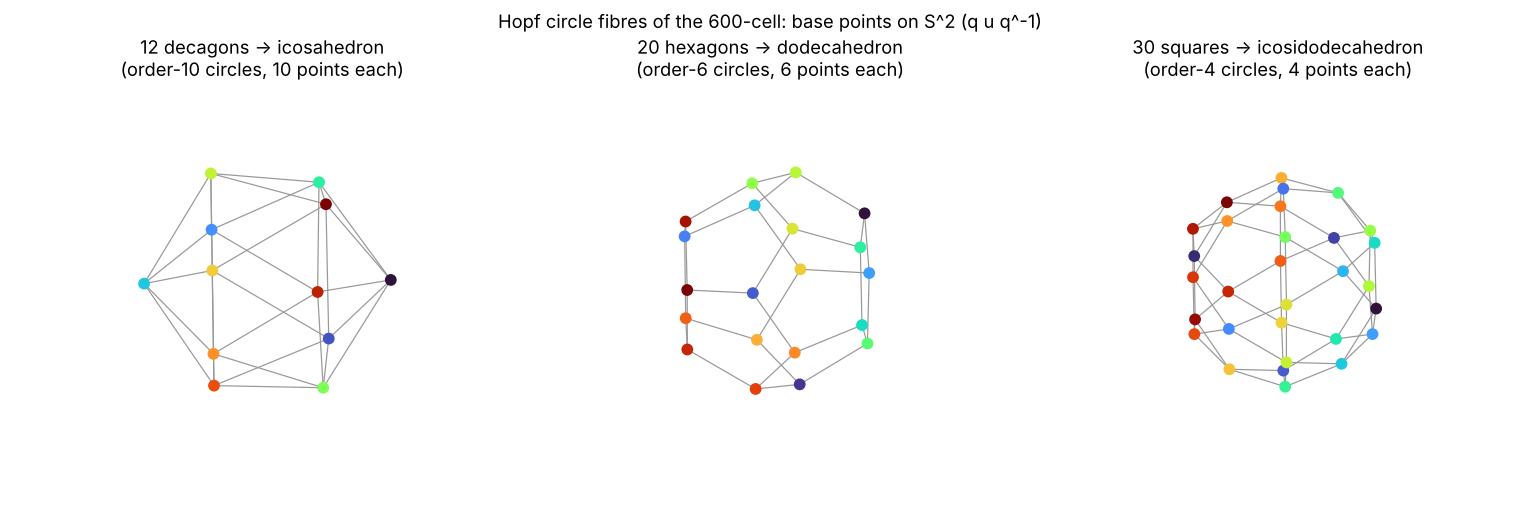
\includegraphics[width=\linewidth]{figures/hopf_shells_600cell.png}
\caption{Hopf circle fibres of the $600$-cell: $12$ decagons, $20$ hexagons and $30$ squares, with base points on $S^2$ (\texttt{models/hopf\_shells.py}).}\label{fig:cells}
\end{figure}

\subsection{Shells and fibres}\label{sec:shells}
The $n$th shell of $E_8$ has $240\,\sigma_3(n)$ vectors, with $\sigma_3(n)=\sum_{d\mid n}d^3$: \qgShellOne, \qgShellTwo\ and \qgShellThree\ vectors for
$n=1,2,3$. Right multiplication by $2T$ acts on each shell.

\begin{result}[\exact\ for $n\le 8$]\label{res:shells}
In shells $1$ to $8$ there are \qgVecEight\ vectors in \qgFibreEight\ fibres, every fibre containing $24$ vectors: shell $n$ has $10\,\sigma_3(n)$ fibres.
\end{result}

This is a finite check, not a proof for all $n$. A formula for the number of classes in terms of ideal norms in $\mathbb{Z}[\varphi]$, which we
write $120\,S(\alpha)$, was checked on shells $1$ to $6$ and as an integer identity for $n\le 60$; it is stated in the repository, and we do not use it
here. Figure~\ref{fig:shells} shows the shell structure.

\begin{figure}[t]\centering
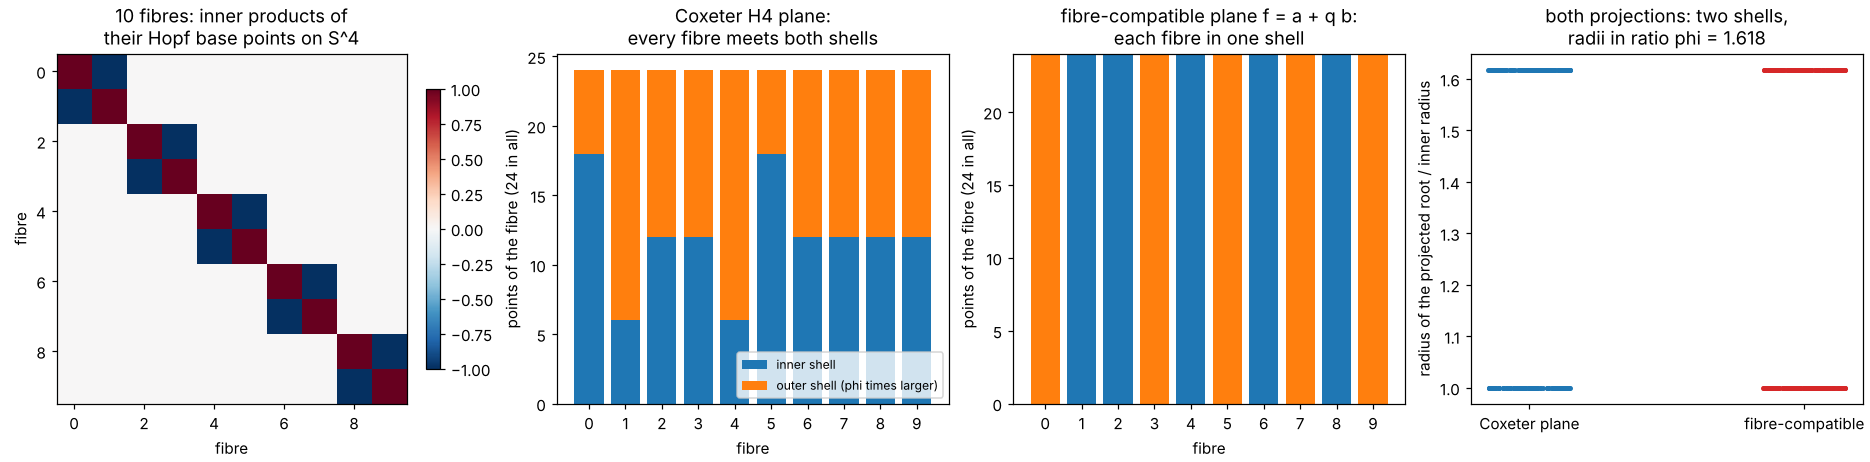
\includegraphics[width=\linewidth]{figures/hopf_shells_e8.png}\\[2pt]
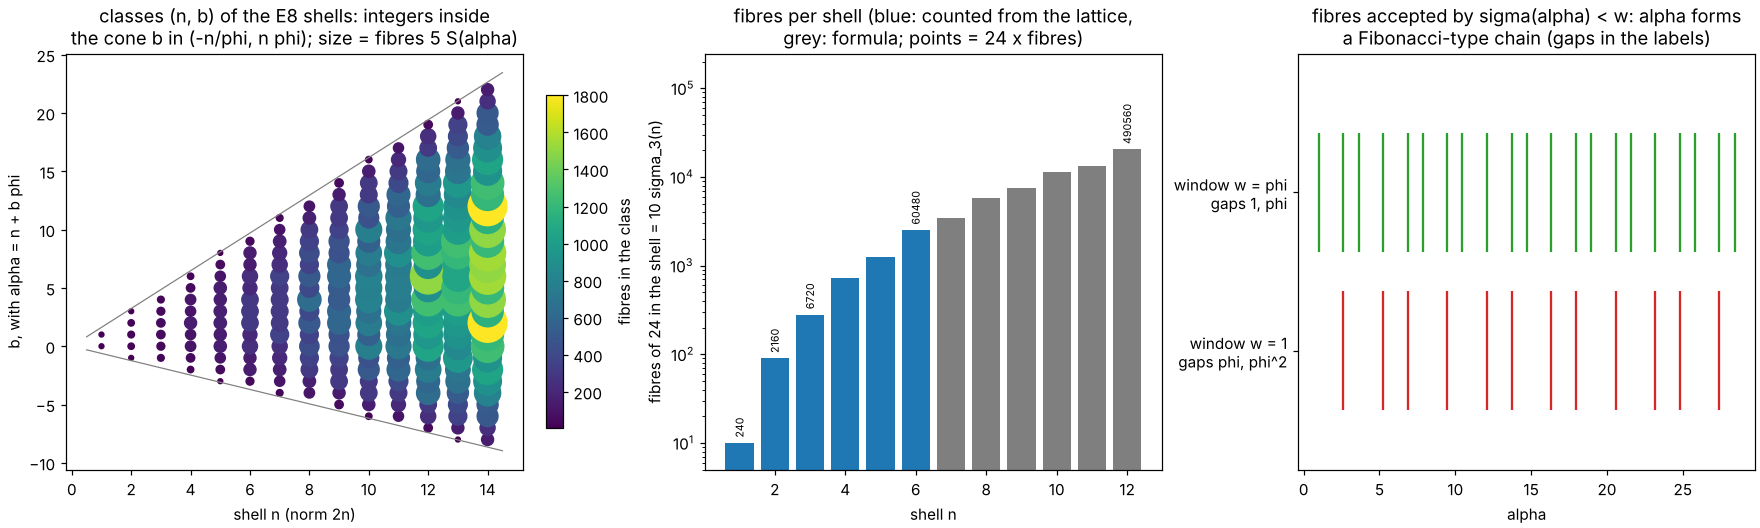
\includegraphics[width=\linewidth]{figures/e8_shells.png}
\caption{Top (\texttt{hopf\_shells.py}): inner products of the base points of the ten fibres; the number of points of each fibre in the two shells of the Coxeter-plane projection and of a fibre-compatible plane; the radii of the two projected shells, in ratio $\varphi$. Bottom (\texttt{e8\_shells.py}): classes $(n,b)$ of the shells; fibres per shell, counted from the lattice (blue, $n\le6$) and from the formula (grey); the accepted classes form a Fibonacci-type chain.}\label{fig:shells}
\end{figure}

\subsection{Windows that keep fibres whole}\label{sec:windows}
A cut-and-project set from $E_8$ keeps the lattice vectors whose perpendicular component lies in a window $W\subset\mathbb{R}^4$. If the construction is
to be organised by fibres, one wants a window that accepts or rejects a fibre as a whole. Whether a window does so depends on the splitting
$\mathbb{R}^8=\mathbb{R}^4_\parallel\oplus\mathbb{R}^4_\perp$ and on the window.

\begin{result}[\exact, shells $1$ to $8$]\label{res:ball}
(i) With the icosian splitting, a ball window $|{\rm perp}|\le R$ splits no fibre, for $R\in\{0.5,0.8,1.0,1.2,1.5,1.8,2.0\}$ (we report
\qgSplitIcosian\ split fibres of \qgFibreEight\ at $R=1.4$). (ii) With the Coxeter-plane splitting, a ball window splits many: \qgSplitCoxOne\ of
\qgFibreEight\ fibres at $R=1.4$ and \qgSplitCoxTwo\ at $R=2.0$.
\end{result}

The reason for (i) is that the fibre rotations act on $\mathbb{R}^4_\perp$ as rotations, so they preserve $|{\rm perp}|$. In the Coxeter-plane splitting
they do not. Both splittings give the same joint distribution of $(|{\rm par}|^2,|{\rm perp}|^2)$ over the vectors, so the distribution does not distinguish them (middle panel of Figure~\ref{fig:windows}, where the two curves coincide).

A natural non-spherical window is the shadow of the Voronoi cell: $W=\mathrm{proj}_\perp(\mathrm{Vor}(E_8))$.

\begin{result}[\exact\ and \numeric]\label{res:vor}
The Voronoi cell of $E_8$ has \qgVoronoiCellVertices\ vertices. In the icosian splitting its perpendicular shadow $W$ is a $4$-polytope with
\qgVoronoiVertices\ vertices and \qgVoronoiFacets\ facets (each with five vertices; the hull routine reports more simplices, because it triangulates),
volume \qgVoronoiVolume, inradius \qgVoronoiIn\ and circumradius \qgVoronoiCirc: it is close to a ball but not a ball. $W$ is invariant under the $24$ fibre rotations, so no fibre
is split: in shells $1$ to $8$, \qgVorAccepted\ of \qgVecEight\ vectors are accepted, in whole fibres. With the Coxeter-plane splitting the same construction splits
\qgVorCoxSplit\ of \qgFibreEight\ fibres. The vertex and facet counts and the radii are computed by a convex-hull routine in floating point (\numeric); the vertex count of the Voronoi cell and
the accept/reject counts are exact integers.
\end{result}

\emph{Proof sketch of the invariance.} Right multiplication by $\ell\in2T$ is a lattice automorphism that commutes with the icosian splitting. It therefore maps $\mathrm{Vor}(E_8)$
to itself, and maps its shadow to itself. The accept/reject rule is ``perp $\in W$'', so it is constant on orbits of $2T$, which are the fibres.
We have not formalised this beyond the sketch; the tests check its consequence on shells $1$ to $8$.

\emph{Attribution.} We believe that this window is the one used by Elser and Sloane, but we have not read their paper, so this is a \hypo, and the result above stands without it.

\begin{figure}[t]\centering
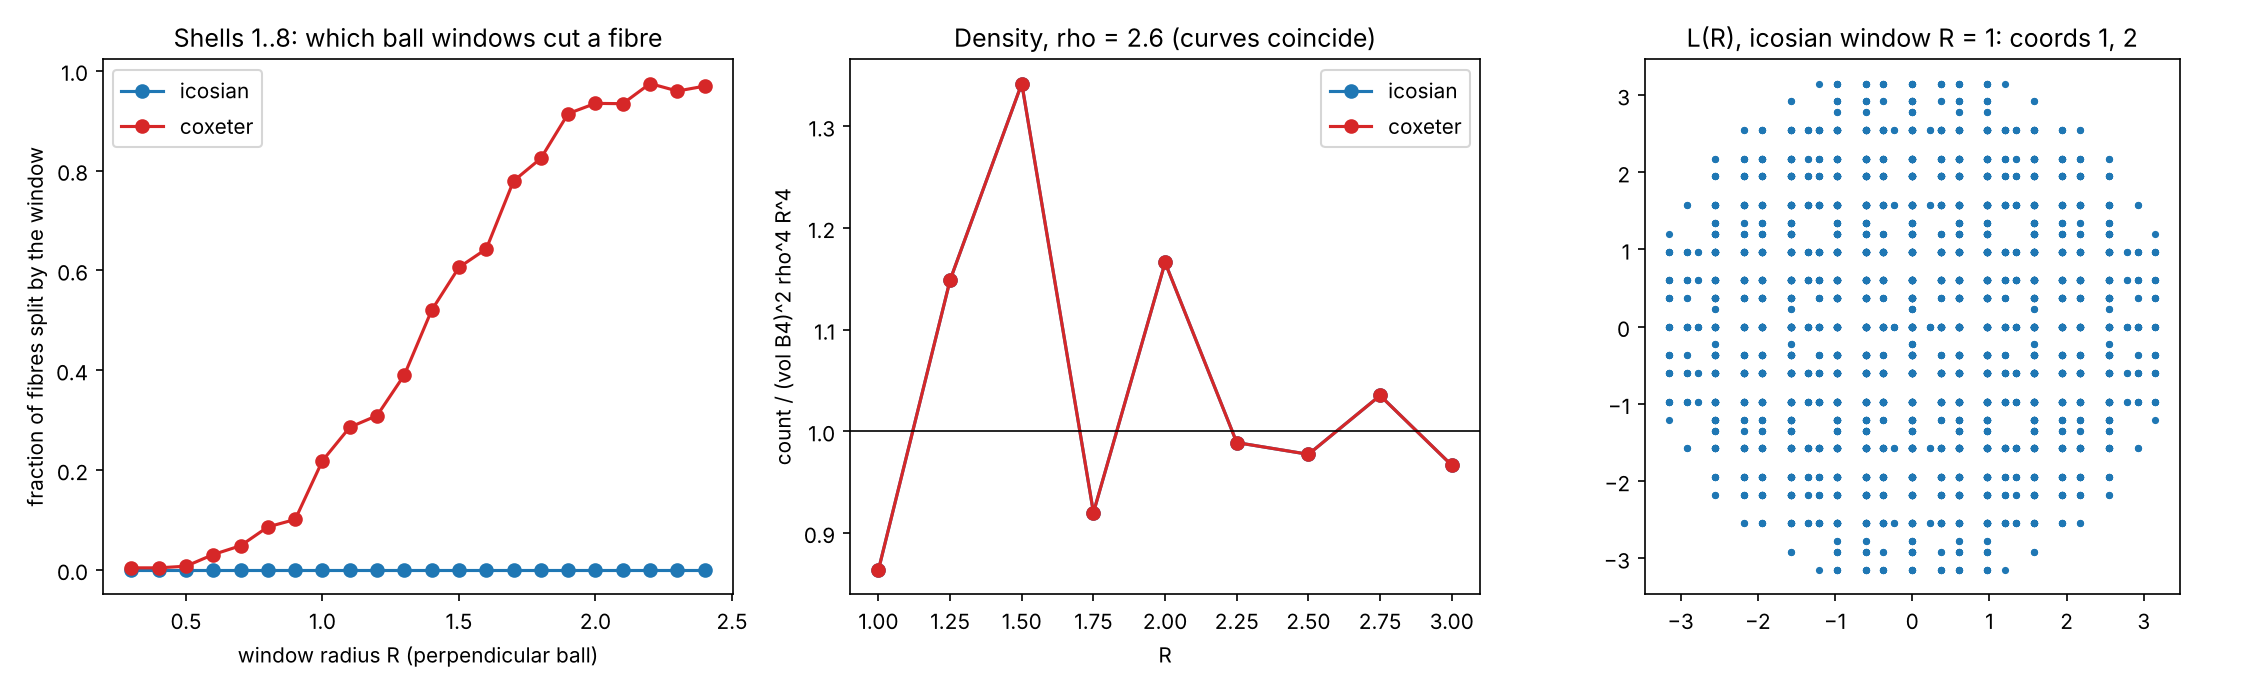
\includegraphics[width=\linewidth]{figures/fibre_window.png}\\[2pt]
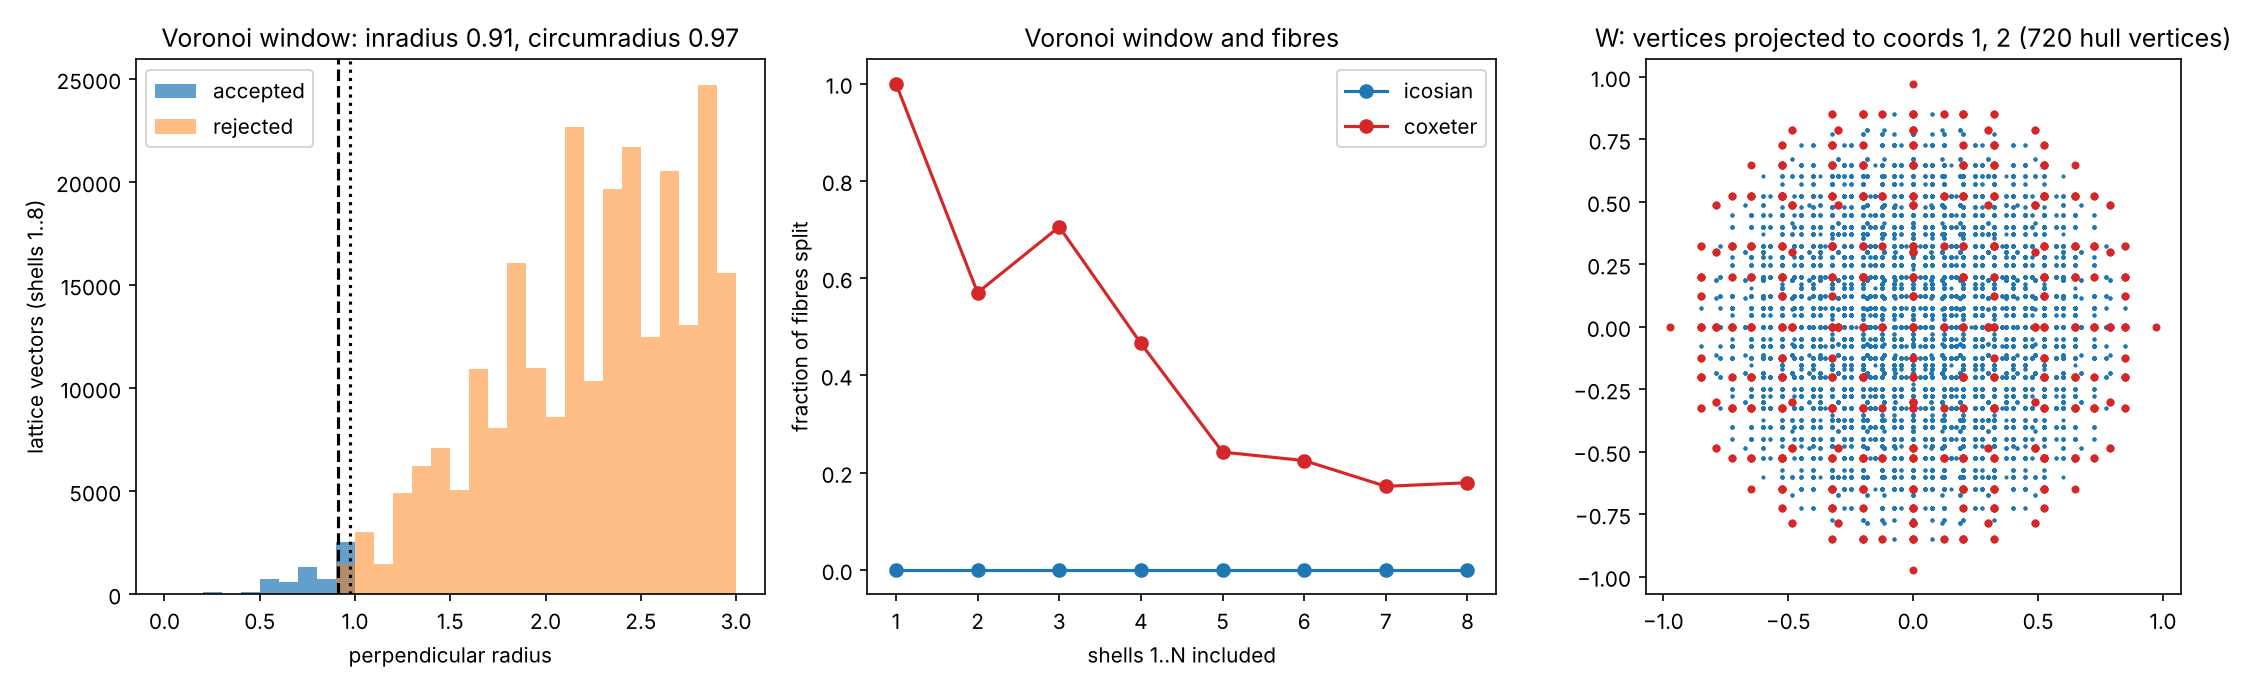
\includegraphics[width=\linewidth]{figures/voronoi_window.png}
\caption{Top (\texttt{fibre\_window.py}): fraction of fibres split by a ball window against $R$ for the two splittings; point density against $R$; the points kept by the icosian window at $R=1$. Bottom (\texttt{voronoi\_window.py}): perpendicular radius of accepted and rejected vectors, with the in- and circumradius of $W$ dashed and dotted; fraction of fibres split against the number of shells included; the vertices of $W$ projected to two coordinates.}\label{fig:windows}
\end{figure}

\subsection{\texorpdfstring{$E_6$}{E6} and the 27}\label{sec:e6}
Inside the fibred root system the two pole fibres, $D_4^a$ and $D_4^b$, are the two $24$-cells with one coordinate zero. The \qgRoots\ roots contain
\qgASubsystems\ subsystems of type $A_2$. Of these, $160$ lie inside one fibre, and $960$ are spread over several fibres.

\begin{result}[\exact]\label{res:e6}
The fibre rotation $R_\omega$ of order $3$ has no fixed vector and permutes the three $64$-root blocks of the $192$ equatorial roots cyclically. The orbit of
$(1+i,0)$ under $R_\omega$ is an $A_2$, and its orthogonal complement in the root system is an $E_6$ with \qgESixRoots\ roots, made of $24+3\times16$ roots. The
\qgRest\ remaining roots form six sets of $27$; each set meets each of the nine fibres other than $D_4^b$ in three roots.
\end{result}

The $E_6\times A_2$ subsystem is a standard feature of $E_8$ (no source was checked for this paper, so none is cited); the content here is only its description in terms of fibres. Figure~\ref{fig:e6} shows it.
\begin{figure}[t]\centering
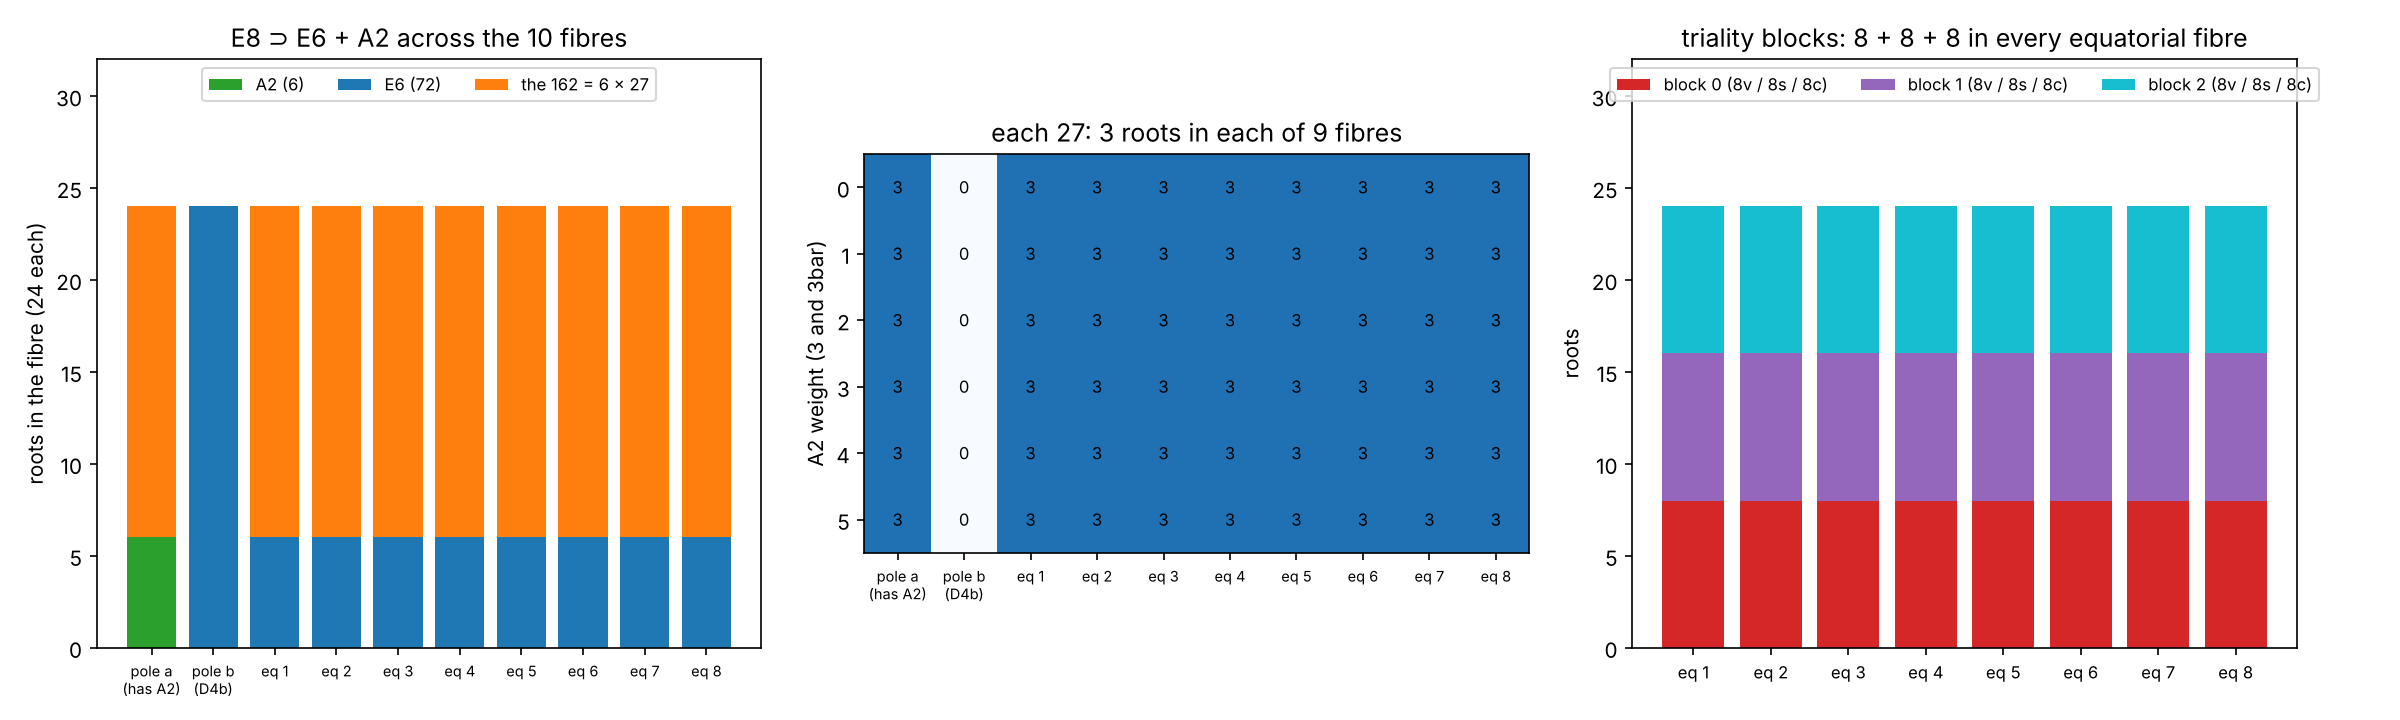
\includegraphics[width=\linewidth]{figures/e6_fibres.png}
\caption{\texttt{e6\_fibres.py}: $A_2$, $E_6$ and the $162=6\times27$ roots in each of the ten fibres; roots of one $27$ in each fibre; the three $8+8+8$ blocks of each equatorial fibre.}\label{fig:e6}
\end{figure}

%------------------------------------------------------------------------------------------------------------------------------------
\section{The Spectre in \texorpdfstring{$E_8$}{E8}}\label{sec:tiles}
\todo{embedding of the lift lattice; every edge a root; patch of \qgTiles\ tiles and \qgVertices\ vertices; corner types $\qgCornersSixty\times60^\circ$, $\qgCornersNinety\times90^\circ$ and $\qgCornersStraight$ straight pass, the same for every tile; edge colours $8+6$ for $\qgTilesMajor$ tiles and $6+8$ for $\qgTilesMinor$ (a rotation by an odd multiple of $30^\circ$ swaps the colours).}
\subsection{The inflation does not extend}\label{sec:inflation}
\todo{\negres: $x^4-8x^2+1$, $\lambda^2=4+\sqrt{15}\approx\qgLambdaSquared$; the field contains $\sqrt{15}$ but not $\sqrt3$, $\sqrt5$ or the golden ratio.}

\section{The Chair44 count}\label{sec:chair}
\todo{\negres: $192=24\times8$ matches the equatorial roots in shape only; which structures fail (negation, free action of order 24).}

%------------------------------------------------------------------------------------------------------------------------------------
\section{An abelian Wilson-loop probe}\label{sec:wilson}
\todo{the programme \cite{peevdogra} needs perimeter and corner extraction; the $U(1)$ Gaussian analogue and what was computed. Results with $\dagger$: aligned fit $\alpha=\qgWAlpha$, $b=\qgWB$ per corner, leave-one-out $\qgWLoo$; failure for a width-3 feature ($\qgWWidthDev$); placement spread $\qgWSpreadlo$ to $\qgWSpreadhi$ and averaged fit $\alpha=\qgWAvgalpha$, $b=\qgWAvgb$; gauge ($\qgWGaugemax$); $L=5$.}
\subsection{What the probe cannot see}
\todo{the hypercubic action treats every turn between different axes as $90^\circ$; the Spectre has $60^\circ$ corners; the Spectre outline written in $\mathbb{Z}^4$ gives $\qgWZfourcornersfirst$ and $\qgWZfourcornerssecond$ corners for the two orderings of its diagonals.}

\section{Open problems and tests that could fail}\label{sec:open}
\todo{from \texttt{TILE\_E8\_BRIDGE.md}, section 3: four tests, none run; the hexagonal action; the choice of placement; larger $L$.}

\appendix
\section{Reproduction}
\todo{table of test modules and counts; the commands; provenance of the snapshot numbers.}
\section{Tight-binding and twist-hopping on the Spectre family}
\todo{short appendix: \texttt{\_tb}, \texttt{chair\_fibers}, \texttt{twist\_hopping}.}

\bibliographystyle{plain}
\bibliography{quantgrav}
\end{document}
